\documentclass{bioinfo}
\usepackage[english]{babel}
\copyrightyear{2015} \pubyear{2015}
\usepackage{natbib}
\bibliographystyle{natbib.bst}


\access{Advance Access Publication Date: Day Month Year}
\appnotes{Manuscript Category}

\renewcommand{\cite}{\citep}
\usepackage{todonotes}

\begin{document}
\firstpage{1}

\subtitle{Subject Section}
\newcommand{\name}{Voodoo }

\title[short Title]{\name: Combining Bottom-up and top-down approaches through graph learning over interaction networks for drug-target-interaction prediction}
\author[Sample \textit{et~al}.]{Tilman Hinnerichs\,$^{\text{\sfb 1,}*}$ and Robert Hoehndorf\,$^{\text{\sfb 2}}$}
\address{$^{\text{\sf 1}}$Department, Institution, City, Post Code, Country and \\
$^{\text{\sf 2}}$Department, Institution, City, Post Code,
Country.}

\corresp{$^\ast$To whom correspondence should be addressed.}

\history{Received on XXXXX; revised on XXXXX; accepted on XXXXX}

\editor{Associate Editor: XXXXXXX}

\abstract{\textbf{Motivation:} Text Text Text Text Text Text Text Text Text Text Text Text Text
Text Text Text Text Text Text Text Text Text Text Text Text Text Text Text Text Text Text Text
Text Text Text Text Text Text Text Text Text Text Text Text Text Text Text Text Text Text Text
Text Text Text Text Text Text
Text Text Text Text Text.\\
\textbf{Results:} Text  Text Text Text Text Text Text Text Text Text  Text Text Text Text Text
Text Text Text Text Text Text Text Text Text Text Text Text Text  Text Text Text Text Text Text\\
\textbf{Availability:} Text  Text Text Text Text Text Text Text Text Text  Text Text Text Text
Text Text Text Text Text Text Text Text Text Text Text Text Text Text  Text\\
\textbf{Contact:} \href{tilman.hinnerichs@kaust.edu.sa}{tilman.hinnerichs@kaust.edu.sa}\\
\textbf{Supplementary information:}10264703 Supplementary data are available at \textit{Bioinformatics}
online.}

\maketitle
\section{Introduction}

In history, traditional remedies, that were known for their medicinal
properties lead to drugs by extraction of the functional
ingredients. Alternatively, characteristics and features of potential
drugs were detected by accident like in the case of penicillin. More
recently, biological drug targets can be found \textit{in silico}
through discovery of suitable computational predictors.

The challenge of accurately predicting drug-target-interactions (DTI)
has shown its importance in the fields of drug repurposing and
repositioning, and in the exploration of novel drugs and their
interaction partners. Knowledge about those links between compounds
and their target proteins help in an array of medical and
pharmaceutical studies. Additionally, those associations can be
utilized to identify disease specific targets, leading to desirable
therapeutic effects.

With the rapidly growing field of machine learning approaches and
their application to bioscientifical problems in the realm of
bioinformatics, different kinds of data, such as long DNA sequences
could be utilized for feature generation, while rapid advances were
made. 

Only recently, the technique of graph learning was introduced by
\citet{GCNConv} through graph convolution algorithms, and improved and
altered under usage of different kernels \cite{ChebConv, ARMAConv},
attention mechanisms \cite{GATConv}, random walks \cite{APPNPConv},
and mixtures of both \cite{SAGEConv}. While based on diverse systems,
they can be relevant for testing distinct hypothesis for given
graphs. While convolutional filters are suitable for finding patterns
among the given graph, attention mechanisms are more relevant for
discovery of important regions within. Lately, graph learning
approaches found application for computing compound representations
for DTI prediction.

These approaches can be classified into top-down and bottom-up methods. Top-down or network approaches hereby start form the observable, phenotypical characteristics, such as side-effects, associated diseases and indications represented by knowledge graphs or ontologies, induced by a drug and infer targets based on the likely molecular mechanisms that result in these phenotypes. On the other hand, bottom-up approaches start from molecular features, such as molecular structure, molecular fingerprints, secondary structure and contact predictions and others, deriving predictions from suitable correlations between these features. 

However, both bottom--up and top--down approaches to drug--target interaction prediction contain some limitations that are not solvable within themselves. Generally, it is very challenging for bottom-up methods to accurately predict, whether there a structure is binding to a protein, as not only molecular structure, but also binding sites and molecular forces are crucial for accurate prediction. Thus, finding similarities for dissimilar drugs affecting the same targets is problematic but crucial. Furthermore, phenotypic features contain relevant information for DTI prediction \cite{Campillos2008} that are complementary to knowledge gained from molecular properties. While bottom-up representations possibly contain all information needed for accurate DTI prediction, we rely on indirect information for better generalization. Contrary, top-down approaches lack the ability to spot and cope with small differences within the molecular drug structure, thus both incapable to predict on novel entities and derive similarity from structural correlation.

In order to design representations concerning both top-down and bottom-up features for proteins and drugs,respectively, we utilize protein--protein interaction (PPI) networks which have shown great results in protein function prediction \cite{Vazquez2003} and antiviral drug--target discovery \cite{Ackerman2019}. 
However, only few applied this context to the task of DTI prediction in humans. The method of graph convolutional neural networks has been applied successfully to PPI networks \cite{Zitnik2017}, granting valuable information for medical diagnostics, closely related to phenotypic information.

Eventually, we further address potential biases and skews within DTI prediction datasets. \todo[inline]{Introduction}
Within DTI prediction, there are potential biases resulting from the
underlying datasets \citep{Pahikkala2014}. First, novel drugs are
often designed by altering non-functional components of a drug,
leading to two and more very similar drugs designed to target the same
proteins \cite{Overington2006}. This can result in a bias when it
leads to hidden duplicates that can distribute among the train/test
split, resulting in a better (measured) predictive performance than
would be expected when the model is applied to identify drugs that
target a protein for which no drugs yet exist. Second, some proteins
(which we call \textit{hub proteins}) have significantly more known
interactions with drugs than others. In the STITCH database, $5\%$ of
the proteins have $40\%$ of the interactions, and similar
distributions are present in the Yamanishi and Drugbank
\cite{Drugbank2007, Drugbank2017} datasets; preferentially predicting
these proteins may increase predictive performance while not
reflecting the actual performance when applied to a new protein (e.g.,
a protein for which no interactions are known). These differences in
the number of drugs targeting certain proteins may be the result of
study bias where more ``valuable'' proteins have more drugs designed
to target them due to their involvement in more common diseases (or
diseases for which drugs can be more profitably marketed). This may affect common \cite{Survey2018} cross-validation splitting schemes, that allow exploitation of these biases within DTI prediction.

\todo[inline]{Somehow smooth this transition}

\enlargethispage{12pt}

\section{Methods}
\subsection{Problem Description}
\name aims to solve the following problem: for a given drug and a
given protein we want to determine whether those interact or not.  We
do not differentiate between types of interaction such as activation
and inhibition, and do not predict the strength of the interaction.
If we additionally assume that our knowledge is complete and all
drug--protein pairs without a known interaction do not interact, we
can formulate the problem as a binary classification task.

\subsection{Datasets}
We obtain a dataset consisting of 12,884 human proteins with over
340627 links from STRING \citep{STRINGv10}. For the drug-target
interactions, we use 229,870 links from the STITCH database
\citep{STITCHv5}. As both STRING and STITCH provide confidence scores
for each association, we filtered them as advised by a threshold of
$700$, therefore retaining only high-confidence interactions.

We utilize the PhenomeNET ontology \citep{PhenomeNET2011}, an ontology
integrating ontologies such as the Human Phenotype Ontology
\citep{HPO2018}, Gene Ontology \cite{GOoriginal2000, GOrecent2020},
Mammalian Phenotype Ontology \citep{MP2009} and several others.
We obtained side effects and their links to drugs from SIDER
\citep{SIDER}; SIDER contains side effects encoded using identifiers
from the MedDRA database \citep{MedDRA}. We mapped side effects to the
PhenomeNET ontology using the \textit{Phenomebrowser.net}, which
provides a SPARQL query endpoint for the mentioned resources.

We only use proteins in our analysis that have at least one link in
either STITCH or STRING, and drugs with at least one side effect and
one existing target. Therefore, the intersection between these
resources yields 1,428 drugs and 7,368 human proteins with 32,212
interactions for the training phase. We provide links to and methods
for obtaining and processing the necessary data on Github.

For comparative evaluation, we use the gold standard dataset
introduced by \citet{Yaminishi2008} consisting of 1,923 interactions
between 708 drugs and 1,512 proteins.
 
\subsection{Model}

Our model combines ``top-down'' and ``bottom-up'' information for
drug--target identification. We consider an approach to be
``top-down'' when observable characteristics of either a drug (such as
a drug effect) or protein (such as a protein function, or phenotypes
resulting from a loss of function) are used to provide information
about a molecular mechanisms; we consider an approach ``bottom-up''
when structural or other molecular information is used to determine a
mechanism.  In order to build a method that incorporates both top-down
and bottom-up features, we first create a model for each type of
feature separately.  As features for the bottom-up model, we use
features derived from molecular structures of drugs from the
\textit{SmilesTransformer} \citep{SmilesTransformer} and molecular
features for proteins from \textit{DeepGOPlus}
\citep{DeepGoPlus}. \textit{SmilesTransformer} introduces an
autoencoder, learning over the SMILES strings and therefore the
molecular organization of each drug in an unsupervised manner. 
\textit{DeepGOPlus} provides features derived from protein amino acid
sequences which are useful to predict protein function.
% Thus, both embeddings seem to suitably supplement
% the following ontology based representations.

As phenotypes and functions are encoded through ontologies, we use
DL2Vec \citep{DL2vec2020} to obtain ontology based representations for
use as top-down features. DL2vec constructs a graph by introducing
nodes for each ontology class and edges for ontology axioms, followed
by random walks starting from each node in the graph. These walks are
encoded using a Word2vec \citep{Word2vec2013} model. Therefore, DL2Vec
generates representations that can encode drug effects or protein
functions while preserving their semantic neighbourhood within that
graph.

% The overall structure of the ontology can be seen in
% Figure~\ref{fig:Onto}.

\todo[inline]{Consider supplement, or combine with other figures.}
\begin{figure}[!tpb]%figure1
	\centerline{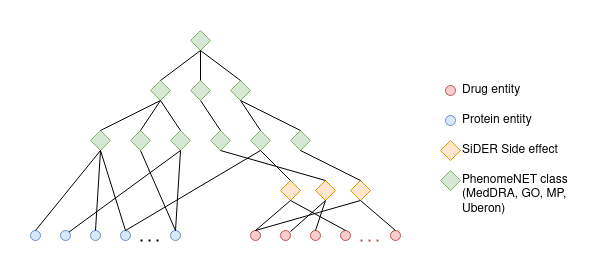
\includegraphics[width=0.5\textwidth]{figures/drug_protein_ontology_network.png}}
	\caption{Drugs and proteins with annotations to SiDER and PhenomeNET}
	\label{fig:Onto}
\end{figure}


\subsubsection{Half-twin neural networks and feature transformation}

As we want to learn from the similarity of drug side effects and
protein phenotypes, we use a deep half-twin neural network with a
contrastive loss using cosine similarity.  A half-twin neural network
aims to learn a similarity between two embeddings of the same
dimension.  The precomputed embeddings may have different
dimensionality and we first process them using a learnable feature
transformation (LFT) network, i.e., a fully connected neural network
layer which takes as input an embedding and outputs a representation
of a particular size. An example structure for both types of features
can be found in Figure~\ref{fig:HalfTwinNetwork}. We use this LFT to
reduce the representation size of the embeddings for drugs and
proteins separately.
% While a regular deep neural network, denoted by LFT, for feature space reduction is not particularly novel, we
The use of an LFT enables flexible experimentation as both ontology
and molecular feature for both drugs and proteins are reduced to
the same dimensionality for varying sizes of inputs; this allows for a
high amount of modularity across different experimental setups by
adding different kinds of features into the model. Additionally, the
generated features may be used for other tasks. % ; for
% example, the ontology LFT can be reused for a variety of DL2vec-based
% features with respect to other ontologies and hypotheses
We follow the results of \textit{DL2vec} \cite{} and use as
activation function $\sigma := \mathrm{LeakyReLU}$ which leads to
improved performance compared to other activation functions.

\begin{figure}[!tpb]%figure1
	\centerline{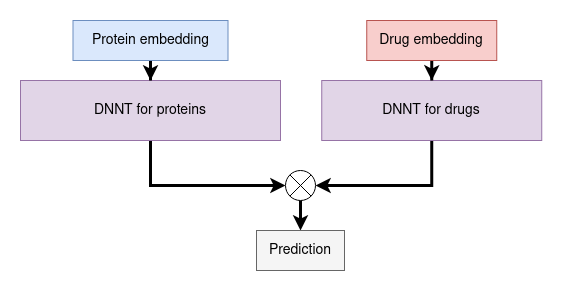
\includegraphics[width=0.35\textwidth]{figures/siamese_network.png}}
	\caption{Half-twin network applied to molecular and DL2vec
          features, utilizing deep learnable feature transformations
          (LFT). The similarity function $\otimes$ yields the
          similarity between both transformed embeddings e.g. by
          computing the cosine similarity.}
	\label{fig:HalfTwinNetwork}
\end{figure}




\subsubsection{Graph convolutional layers}

We include these molecular and ontology-based sub-models within a
graph neural network (GNN). The graph underlying the GNN is based on
the protein--protein interaction (PPI) graph. The PPI dataset is
represented by a graph $G=(V,E)$, where each protein is represented by
a vertex $v\in V$, and each edge $e\in E\subseteq V\times V$
represents an interaction between two proteins. Additionally, we
introduce a mapping $x:V\rightarrow\mathbb{R}^{d}$ projecting each
vertex $v$ to its node feature $x_v := x(v)$, where $d$ denotes the
dimensionality of the node features.
 
% As described before, graph convolution has shown significant
% performance increase in a variety of tasks. While there are various
% methods out there we will only introduce the most basic one here. 
A graph convolutional layer \cite{GCNConv} consists of a learnable
weight matrix followed by an aggregation step, formalized by
\begin{equation}
	\mathbf{X}^{\prime} = \mathbf{\hat{D}}^{-1/2} \mathbf{\hat{A}}
	\mathbf{\hat{D}}^{-1/2} \mathbf{X} \mathbf{\Theta}
\end{equation}
where for a given graph $G=(V,E)$, $\hat{A} = A + I$ denotes the
adjacency matrix with added self-loops for each vertex, $D$ is
described by $\hat{D}_{ii} = \sum_{j=0} \hat{A}_{ij}$, a diagonal
matrix displaying the degree of each node, and $\Theta$ denotes the
learnable weight matrix. Added self-loops enforce that each node
representation is directly dependent on its own preceding one. The
number of graph convolutional layers stacked equals the radius of
relevant nodes for each vertex within the graph.

The update rule for each node is given by a message passing scheme
formalized by
\begin{equation}
	\mathbf{x}^{\prime}_i = \mathbf{\Theta} \sum^{N}_{j}
	\frac{1}{\sqrt{\hat{d}_j \hat{d}_i}} \mathbf{x}_j
\end{equation}
where both $\hat{d}_i, \hat{d}_j$ are dependent on the edge weights
$e_{ij}$ of the graph. With simple, single-valued edge weights such as
$e_{ij}=1 \text{ }\forall (i,j)\in E$, all $\hat{d}_i$ reduce to
$d_i$, i.e., the degree of each vertex $i$. We denote this type of
graph convolutional neural layers with \textsc{GCNConv}.

While in this initial formulation of a GCNConv the node-wise update
step is defined by the sum over all neighbouring node representations,
we can alter this formulation to other message passing schemes.  We
can rearrange the order of activation function $\sigma$, aggregation
$\mathrm{AGG}$, and linear neural layer $\mathrm{MLP}$ with this
formulation as proposed by \citet{GENConv2020}:
\begin{equation}
	\mathbf{x}_i^{\prime} = \mathrm{MLP} \left( \mathbf{x}_i +
	\mathrm{AGG} \left( \left\{
	\mathrm{\sigma} \left( \mathbf{x}_j + \mathbf{e_{ji}} \right) +\epsilon
	: j \in \mathcal{N}(i) \right\} \right)
	\right)
\end{equation}
where we only consider
$\sigma \in \{\mathrm{ReLU}, \mathrm{LeakyReLU}\}$. We denote
this generalized layer type as \textsc{GENConv} following the
notation of PyTorch Geometric \cite{PytorchGeometric}.  While the
reordering is mainly import for numerical stability, this alteration
also addresses the vanishing gradient problem for deeper convolutional
networks \cite{GENConv2020}. Additionally, we can also generalize the
aggregation function to allow different weighting functions such as
learnable $\mathrm{SoftMax}$ or $\mathrm{Power}$ for the incoming
signals for each vertex, substituting the averaging step in
\textsc{GCNConv}. Hence, while \textsc{GCNConv} suffers from both
vanishing gradients and signal fading for large scale and highly
connected graphs, each propagation step in \textsc{GENConv} emphasizes
signals with values close to $0$ and $1$. The same convolutional
filter and weight matrix are applied to and learned for all nodes
simultaneously. % , and the resulting information\todo{Which information?
  % Specify} hold no information on their own connectivity.
We further employ another mechanism to avoid redundancy and fading
signals in stacked graph convolutional networks, using residual
connections and a normalization scheme \cite{DeepGCN2019,
  DeeperGCN2020}.  The residual blocks are reusable and can be stacked
multiple times. The structure of the GNN architecture we use is shown
in Figure~\ref{fig:ResGraphConvBlocks}.

\begin{figure}[!tpb]%figure1
	\centerline{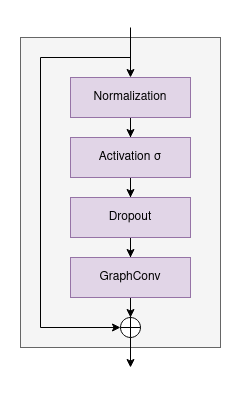
\includegraphics[width=0.5\columnwidth]{figures/ResGraphConvBlocks.png}}
	\caption{Residual architecture built by \citet{DeepGCN2019} and \citet{DeeperGCN2020} enabling deeper graph convolutional models}
	\label{fig:ResGraphConvBlocks}
\end{figure}


\begin{figure}[!tpb]%figure1
	\centerline{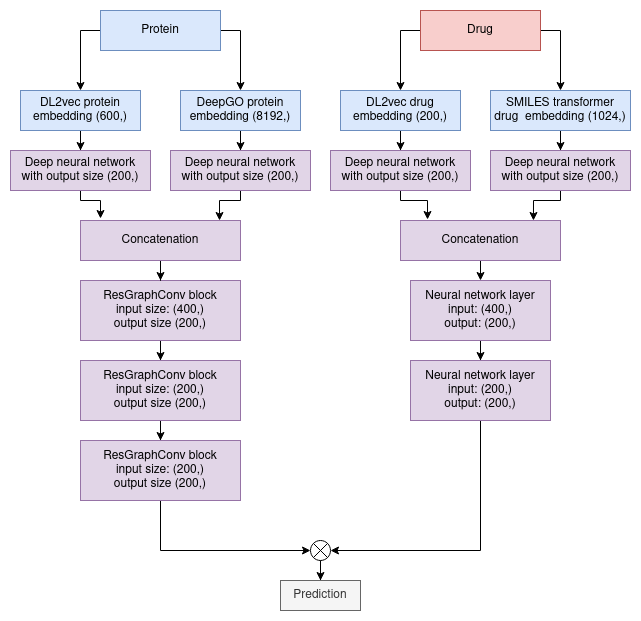
\includegraphics[width=1\columnwidth]{figures/full_model_all_layers.png}}
	\caption{Residual architecture built by \citet{DeepGCN2019} and \citet{DeeperGCN2020} enabling deeper graph convolutional models}
	\label{fig:FullModelAllLayers}
\end{figure}

\subsubsection{Combined prediction model}
Combining half-twin and graph convolutional neural networks, we map
all protein representations to their respective node features,
initializing the graph convolutional update steps. The resulting
representations are used for a similarity prediction as presented in figure ~\ref{fig:HalfTwinNetwork}. 
When combining ontology and molecular features with or without the
graph model, we concatenate both protein features and both drugs
features, before plugging them into the graph model for the similarity
computation. A more in-depth image of the overall and final architecture,
combining both feature types, is depicted in figure
~\ref{fig:FullModelAllLayers}. Here the original representations are transformed by LFTs and then run through a stack (here with height 3) of residual graph convolutional blocks.

\subsubsection{Hyperparameter tuning}
As the number of drug-targets are sparse with respect to the number of
both drugs and proteins considered, the training, validation and
testing datasets are imbalanced. As there are only $22,336$ links in
the considered STITCH subset, the ratio
\begin{equation}
	w:= \frac{\#drugs \cdot \#proteins}{\#dti\_links} \approx 360,
	\label{weight}
\end{equation}
consequently needs suitable compensation in the computed loss function and
appropriate metrics for the evaluation.

Therefore, we weight all positive drug-protein pair samples with this
ratio by introducing the following loss function with respect to 
binary cross-entropy:
\begin{equation}
	l(x,y) = - w \left[ y \cdot \log x + (1 - y) \cdot \log (1 - x) \right]
\end{equation}
for a given prediction $x$ and target $y$, and positive weight $w$
defined by equation \eqref{weight}. We average this loss among all
drug-protein pairs in the training set, leading to a stable
environment for the \textit{Adam} optimization algorithm
\citep{Adam2014}. We implemented a 5-fold cross validation split among
the proteins. Furthermore, we used early stopping in the training
process.

To find the best hyperparameter configuration for the proposed model,
we performed a grid search to find the most expressive and
non-redundant representation. We pretrained the bottom-up and the
top-down model separately and aimed at best performing models
with respect to our evaluation metrics. We optimized embedding sizes,
depth of the neural network, optimizer, learning rate and layer types
using an extensive, manual grid search. Starting from na\"ive, shallow
feature transformations with an embedding size of $10$, we scaled the
network up to residual structures with up to $10$ hidden layers
leading to embeddings of size $4000$, testing different network widths
and learning rates for each configuration.

\subsection{Evaluation and metrics}
\label{sec:evaluation}
To assess each model, we compute a variety of common metrics for
binary classification. As the datasets are highly imbalanced, we use
the area under the receiver operating characteristic curve
(AUROC) on training, validation and testing split. % We
% calculated the true positive rate (TPR), false positive rate (FPR), and
% precision score. We will further compute true positives (TP), false
% positives (FP), false negatives (FN) and finally true negatives (TN).

We calculate the AUROC by computing true positive rate at various
false positive rate thresholds and use trapezoidal approximations to
estimate the area under the curve. We refer to this measure as
$\textrm{MacroAUC}$.

\todo[inline]{For RH: check this again later:}
We also calculate the $\textrm{MicroAUC}$ score. For given lists $D$
and $P$ of drugs and proteins, respectively, and a set of known
interactions $Int := \{(d_i, p_i) \}$, \textit{MicroAUC} is calculated
as the average per entity (macro) \textit{AUROC} score. Specifically,
for protein-centric score, this can be formalized as: given labels
$l:D\times P \rightarrow \{0,1\}$ and predictions $y:D\times P
\rightarrow [0,1]$, we define
\begin{equation*}
  \textrm{MicroAUC}'_p(l,y) := \underset{p\in P}{mean}\left(\left\{
      \text{AUROC}(\{ (l(d_i, p), y(d_i,p))| d_i\in D\})
    \right\}\right)
\end{equation*}

In some cases, the $MicroAUC'$ score may not be defined as in some
datasets some proteins or drugs have no interactions, leading to an
infeasible $TPR=0$ for all thresholds and an undefined $AUROC$ score
for that entity. For those entities, we impute the $MicroAUC$
interpolating linearly, by using the accuracy for this
subset:

\begin{equation*}
	\textrm{MicroAUC}_p(l,y) := 
	\begin{cases}
		MicroAUC'_p(l,y) & \text{if }\sum_{d_i\in D}l(d_i,p)\neq0\\
		Accuracy(l,y)&otherwise
	\end{cases}
\end{equation*}

Note that drugs and proteins can be interchanged in this formulation, and we
refer to the different measures as protein-centric microAUC
($MicroAUC_p$) and a drug-centric microAUC ($MicroAUC_d$).



\section{Results}

\subsection{\name: computational model to identify drugs that target a
  protein}

% As in machine learning inference is derived from the underlying data,
% models and data are naturally and intrinsically linked. Thus, the more
% we understand about the pitfalls and biases within the data, the more
% we can try to bypass these difficulties. We will hereby abbreviate,
% e.g., a cross validation splitting scheme as \glqq split\grqq{}
% determining the train, validation and test subset of a given dataset.

We developed \name as a computational model to predict drug--target
interactions. Specifically, given a protein, \name will identify and
rank drugs that likely target this protein. \name combines two types
of features: structural information for drugs and proteins that can be
used to determine if the drug and protein physically interact, and
information about phenotypic effects of drugs and changes in protein
function that may ``localize'' on an interaction network (i.e.,
neighboring nodes will share some of these features or are
phenotypically similar).  As structural features, \name uses
structural representations of drugs from the SMILES transformer
\cite{SmilesTransformer} and representations of protein amino acid
sequences from DeepGOPlus \cite{DeepGoPlus}.  \name learns
representations of drug effects and protein functions using the
ontology-based machine learning method DL2Vec \cite{DL2vec2020} and
ontology-based annotations of drugs and proteins.

We construct a graph with proteins as nodes and protein-protein
interactions as edges, mapping the protein features to each target as
node features. \name then propagates information among the PPI network
utilizing graph convolutional steps, calculates the similarity of drug
and protein representations, and predicts whether there is an
interaction. The full workflow scheme is depicted in
figure~\ref{fig:ModelWorkflow}

% Note that this approach can be easily generalized, profiting from
% other protein function and phenotype representation methods.


\begin{figure}[!tpb]
	\centering
	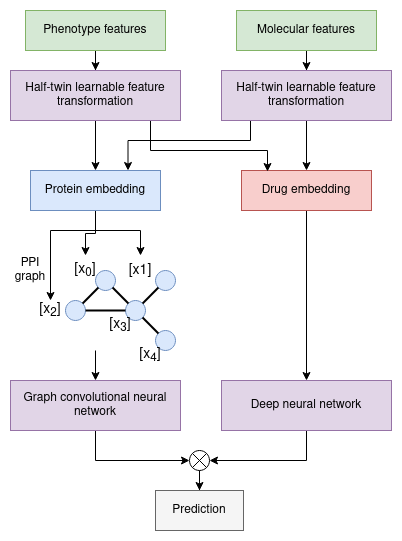
\includegraphics[width=0.9\columnwidth]{figures/model_workflow.png}
	\caption{Full DTI prediction model based on the pretrained
          learnable feature transformations (LFT) for either molecular
          structure or ontology based features. The transformed
          protein representations are added to each corresponded
          protein as node features for the graph convolutional
          steps.}
	\label{fig:ModelWorkflow}
\end{figure}

\begin{table*}[!tpb]
  \centering
	\begin{tabular}{|p{2.2cm}|p{0.9cm}|p{0.75cm}|p{0.9cm}|p{0.75cm}|p{0.9cm}|p{0.75cm}|p{0.9cm}|p{0.75cm}|}
		\hline
		&\multicolumn{4}{c|}{(a) STITCH results}& \multicolumn{4}{c|}{(b) Yamanishi results}\\
		\hline
		\name results&\multicolumn{4}{c|}{PPI graph}&\multicolumn{4}{c|}{PPI graph}\\
		&\multicolumn{2}{c|}{without}&\multicolumn{2}{c|}{with}&\multicolumn{2}{c|}{without}&\multicolumn{2}{c|}{with}\\
		&Macro AUC&Micro $AUC_p$&Macro AUC&Micro $AUC_p$&Macro AUC&Micro AUC&Macro AUC&Micro $AUC_p$\\
		\hline
		MolPred&$0.69$&$0.65$&$0.69$&$0.67$&$0.66$&$0.67$&$0.66$&$0.64$\\
		\hline
		OntoPred&$0.88$&$0.87$&$0.92$&$0.93$&$0.80$&$0.79$&$0.83$&$0.82$\\
		\hline
		\name (MolPred + OntoPred) & $0.89$ & $0.90$&$\mathbf{0.93}$&$\mathbf{0.94}$& $0.83$ & $0.82$&$\mathbf{0.84}$&$\mathbf{0.84}$\\
		\hline
	\end{tabular} \medskip

	\begin{tabular}{|l|p{1cm}|p{1cm}|p{1cm}|p{1cm}|}
		\hline
		(c) Approach&\multicolumn{2}{c|}{Original scheme}&\multicolumn{2}{c|}{Protein split}\\
		&Splitting scheme&Macro AUC&Macro AUC&Micro $AUC_p$\\
		\hline
		Naive predictor&DP pairs&$0.85$& --&--\\
		DTINet&DP pairs&$0.91$&$0.74$&$0.67$\\
		DTIGEMS+&DP pairs&$\mathbf{0.93}$& $0.72$& $0.68$ \\
		DTI-CDF&Proteins&$0.85$&$\mathbf{0.85}$&$0.79$\\
		\name&Proteins&$0.84$&$0.84$&$\mathbf{0.84}$\\
		\hline
		\hline
		(d) Approach&\multicolumn{2}{c|}{Original scheme}&\multicolumn{2}{c|}{Protein split}\\
		&Splitting scheme&Macro AUC&Macro AUC&Micro $AUC_p$\\
		\hline
		Naive predictor&DP pairs&$0.79$&-- &--\\
		DeepDTI&Drugs&$0.88$&$0.76$&$0.70$\\
		DeepDTA&DP pairs&$0.88$&$0.77$&$0.69$\\
		DeepConv-DTI&DP pairs&$0.88$&$0.76$&$0.73$\\
		MolTrans&DP pairs&$0.90$&$0.77$&$0.74$\\
		\hline
	\end{tabular}\\
	
	\caption{(a) + (b) Results for \name on STITCH and Yamanishi dataset evaluated with a 5-fold cross-validation. We hereby denote the molecular feature based predictor with \textit{MolPred}, while abbreviating the ontology based, top-down predictor with \textit{OntoPred}. (c) + (d) Results for various state of the art (c) drug--target interaction prediction methods on Yamanishi dataset and (d) drug--target affinity prediction methods on BIOSNAP dataset, evaluated on their original and the protein cross-validation splitting scheme, approximately reproducing the results of MolTrans \textbf{CITATION}.}
	\label{tab:Results}
\end{table*}

We evaluate our model's ability to identify drug--target interactions
using different approaches and datasets. First, we perform a
cross-validation over proteins and validate our results. A
cross-validation over proteins aims to evaluate how the model performs
when tasked to identify drugs that may target a ``novel'' protein,
i.e., one not seen during training, or a protein for which a drug that
targets it should be predicted. 

We trained, validated and finally tested all considered models on the
STITCH dataset using a 5-fold cross-validation over a protein split;
we then selected the best-performing models (with respect to $MicroAUC_p$,
see Section \ref{sec:evaluation}) and evaluate them in a 5-fold
protein-split cross-validation on the Yamanishi benchmark dataset to
avoid validation overfitting and yield more realistic testing
results. To evaluate the influence of the different features
separately, and to determine whether they ``localize'' on the PPI
graph (and therefore can be exploited successfully by the graph neural
networks), we train and evaluate models with different types of
features, and with and without inclusion of the PPI graph,
separately. We comparing the molecular (MolPred) and phenotype-based
(OntoPred) prediction model, and a combination of both where we
concatenate both types of features.  Table
\ref{tab:Results}\todo{check -- not currently in the table} shows the
results of these experiments.

We find that the model using ontology-based features
(\textit{OntoPred}) is showing better performance on STITCH compared
to using only molecular features. We also observe that only the model
using ontology-based features results in increased performance when
incorporating the PPI graph. This increase can be observed with
different graph neural network architectures and configurations. While
the {\em GCNConv} and {\em GENConv} architecture already shows some
minor improvement, the use of \textit{ResGraphConv} results in larger
performance improvements.  {\em ResGraphConv} blocks add a large
amount of additional learnable parameters to the network, leading to
more expressive power. To test whether the observed improvement is due
to the number of learnable parameters added or the result of better
exploiting the information about PPIs, we experiment with a graph
model in which all graph convolutional neural layers in the residual
blocks are removed, resulting in a model with similar parameters but
without the ability to use graph-based information. This pruned
network, with no information on the protein--protein interactions,
reached very similar results to the original \textit{OntoPred} model
and showed no improvement.

The improvements when including the graph are only provided by the
\textit{GENConv} graph convolution scheme which includes the
{\em ResGraphConv} blocks; \textit{GCNConv} and other graph
convolutional methods fail to achieve any gain in comparison to the
plain \textit{OntoPred} performance even when combined with the
residual blocks. The discrepancy between {\em GENConv} and other graph
convolutional methods may be the result of numerical instability and
fading signals \cite{}.

Our results demonstrate that the inclusion of graph information
can increase performance when ontology-based features are used but not
when molecular features are used alone. This observation allows us to
conclude that information about protein functions localizes on the
graph whereas molecular features do not.

% despite predicting per protein is
% rather counter-intuitive as there only limited drug-targets
% \citep{Overington2006}, and thus novel drugs are more likely to arise
% than novel targets. Yet, we aim to find all interacting drugs for
% existing targets motivating our split choice even further.




\subsection{Protein-centric evaluation}
The goal of \name is to find candidate drugs that target a specific
protein; however, so far, we do not evaluate this application but
rather how \name would perform in finding plausible drug--target
interactions among all possible interactions (since we use the
MacroAUC as our main evaluation measure). This evaluation does not
correspond to the application of \name in finding drugs that target a
specific protein.  To provide a better estimate on how \name performs
for individual protein targets, we use micro-averages between proteins
and compute the \textit{MicroAUC} (see Section \ref{sec:evaluation});
to determine {\em MicroAUC}, we average the performance (true and
false positive rates) per protein instead of across all drug--protein
pairs; the resulting measure can therefore better estimate how \name
performs when tasked with finding a drug that targets a specific
protein.

% Note, that both $MicroAUC_p$ and $MicroAUC_d$, as introduced in the previous chapter, are applicable to all three kinds of splitting schemes, but $MicroAUC_p$ and $MicroAUC_d$ are most plausible and valuable for protein split and drug split, respectively. As we want to evaluate the models performance to find all suitable drugs for each protein individually, \textit{$MicroAUC_p$} seems to be more reasonable in comparison to both $MicroAUC_d$ and $AUROC$ with respect to the previously proposed protein split cross-validation. 


% \subsection{Baseline model}
Furthermore, we hypothesize that it may be possible to exploit biases
in drug--target interactions to achieve relatively high prediction
performance without obtaining a biologically meaningful signal.
For example, hub proteins may have a large number of interactions,
or certain drugs interact with many proteins, and preferentially
predicting these interactions may increase predictive performance even
in the absence of any biological features.
To test this hypothesis, we design a ``na\"ive'' baseline model that
predicts the same list of proteins for each drug based only on the
number of known drug--target interactions for a protein. Formally,
given lists $D$ and $P$ of drugs and proteins and a set of known
interactions $\mathcal{I} := \{(d_i, p_i) \}$, we construct an
interaction matrix $M_{int}\in\{0,1\}^{|D|\times|P|}$ with
\begin{equation*}
	M_{ij} = \begin{cases}
		1 & \text{if } (d_i, p_j)\in \mathcal{I}\\
		0 & otherwise
	\end{cases}
\end{equation*}
describing for all drug--protein pairs whether there is a known
interaction or not. We now rank all proteins $p_j\in P$ descending by
their number of drug interactors by summing over the columns of
$M_{ij}$ and ranking these sums:
\begin{equation*}
	f: P \rightarrow \mathbb{N} \text{ with } f:p_j \mapsto \sum_{i=1}^{|D|}M_{ij}
\end{equation*}
Our ``na\"ive'' predictor $P_k$ predicts all drugs to interact with
the top $k$ targets with respect to the introduced ranking:
\begin{equation*}
	P_k: D\times P \rightarrow \{0,1\} \text{ with } P_k: d_i, p_j \mapsto \begin{cases}
		1 & \text{ if }p_j \in Top_{k}(P)\\
		0 & otherwise
	\end{cases}
\end{equation*}
with the only hyperparameter $k$.

The prediction $P_k$ is not dependent on the drug $d_i$ and will
predict the same ranked list of drugs for all proteins; consequently,
this na\"ive predictor does not rely on any biological features and
will not predict any novel information about interactions between
drugs and proteins; the na\"ive predictor only exploits imbalances in
the evaluation set to make predictions that may perform
well. % but allows us to estimate the effect of potential
% biases in our evaluation dataset.
% Also note the possibility for a similar predictor by calculating the top $k$ interacting drugs, respectively.

The way in which we formulated the na\"ive predictor, it is not
applicable for a protein split cross-validation as the number of
interactions for each protein in the validation set is unknown.  We
apply this naive predictor on both the STITCH and Yamanishi datasets,
using the full datasets as well as a 5-fold cross-validation over
drugs and over drug--protein pairs to compare the prediction results
directly to \name.  For each fold, we gradually increase $k$ to
determine the best performance for each fold. Using the full dataset,
drug--target split, and drug split, we obtain the following MacroAUC
results\todo[inline]{Put in Results table, then remove from here}: for
the STITCH database, we obtain a performance of $0.76$ on the whole
dataset, $0.70$ for the drug--target pairs and $0.73$ in case of the
drug splitting scheme; on the Yamanishi dataset, we obtain MacroAUC
scores of $0.88$, $0.84$ and $0.85$, for the total dataset,
drug--target pair and drug split, respectively.  The na\"ive predictor
shows higher performance on the Yamanishi dataset than on STITCH, and
a substantial gain in comparison to an expected random predictor on
both datasets. In the following, we utilize this nai\"ve predictor as
baseline to compare its performance to state of the art models and
\name.

For comparison with the state of the art methods, we chose the best
performing methods for drug--target interaction prediction that were
previously evaluated on the Yamanishi benchmark dataset. These methods
include DTIGEMS+ \cite{DTIGEMS2020} and DTI-CDF \cite{DTI-CDF2019}
which have showed superior results in comparison to numerous
works. Furthermore, we added DTINet \cite{DTINet2017} as method for
comparison which has been used to develop a number of methods such as
NeoDTI \cite{NeoDTI2019} with similar methodology.

We evaluate all models on their recommended splitting scheme choice,
hyperparameters and folds in cross-validation, measuring their
respective AUROC. We further evaluate each model by performing a
protein-wise cross-validation determining the MacroAUC and
$MicroAUC_p$. For this evaluation, we allow
sub-sampling of negatives for the training process
but not for the validation and testing phase as real world
applications of these models would have to deal with possibly
imbalanced data.

The results of our experiments are summarized in part (c) of Table
\ref{tab:Results}\todo{Check after restructure}; we calculated the
performance of all compared methods over their original splitting
scheme and over a protein split. We find that there is a large
difference in performance when evaluating over a drug--target pair
split compared to a protein split, with generally higher performance
achieved when using the drug--target pair split.  Second, when
evaluating the same methods over a protein split, we find a
substantial performance difference in comparison to the splitting
scheme used in the original evaluation of each method. DTI-CDF was
originally evaluated on all three splitting schemes underlining this
point \cite{}. While \name provides comparable performance to the
na\"ive predictor and DTI-CDF in terms of MacroAUC, it yields
considerably better results with respect to $\textrm{MicroAUC}_p$. We
also find that methods that are trained using a protein split
generally result in higher $\textrm{MicroAUC}_p$ than methods trained
using a drug--target pair split.

As the difference in performance with different splitting schemes is
quite large, we further evaluated additional drug--target interaction
and drug--target affinity prediction methods that were trained and
evaluation on other datasets.  Following the results of MolTrans
\cite{MolTrans2020}, we reevaluated DeepDTI \cite{DeepDTI2017}, DeepDTA
\cite{DeepDTA2018}, DeepConv-DTI \cite{DeepConvDTI2019} and MolTrans itself on BioSnap\todo{What
  is that? Is it described in methods?}  \cite{} over a protein split,
as shown in part (d) of Table \ref{tab:Results}\todo{check table}. The
authors of MolTrans evaluated all considered methods over the
drug--target pair and the protein split; we were able to reproduce the
results (Table \ref{tab:Results} (d))\todo{check table}, showing a
substantial difference based on the splitting scheme. We additionally
computed the $MicroAUC_p$ score for all considered methods, leading to
evaluation results that are comparable\todo{are the datasets
  comparable?} to the ones obtained on the Yaminishi dataset.

\todo[inline]{ add \name model to table to allow
  DIRECT comparison:}
The results of the analysis are summarized in the upper part of Figure
\ref{tab:Results}.

We find that...\todo[inline]{summarize key findings from Table.}


\todo[inline]{Replace/merge table:}


%As the baseline predictor is based on the second dataset bias i.e. the existence of hub proteins with significantly more interactions within the dataset, this may hint on a more severe skew within the Yamanishi benchmark. 




\section{Discussion}

\subsection{``Bottom-up'' and ``top-down'' prediction of drug-target interactions}

There are many computational methods to predict drug--target
interactions. They can broadly be grouped in two types; the first,
which we refer to as ``bottom-up'' approaches, start from molecular
information about a drug and protein and predict an interaction based
on their molecular properties; the second, which we refer to as
``top-down'' approaches, start from observable characteristics of an
organism and infer drug--target interactions as the putative molecular
mechanisms that explain these observations; many top-down approaches
follow methods similar to those used in reverse genetics \cite{}.

Another view on these two approaches is as direct and indirect ways to
predict drug--target interactions. Molecular information can be used
to directly determine whether two molecules (such as a drug and
protein) have the ability to interact, whereas information about
phenotypic consequences of a drug (drug effects) or disruption of a
protein function can be used to indirectly suggest candidate
drug--target interactions. Molecular information will be specific to a
drug--target pair and we would not expect this information to
propagate through a protein--protein interaction network; the main
information about drug--target interactions that could be obtained
from interactions between proteins is information about binding sites
between proteins that may also be used by a drug molecule (i.e.,
information that protein $P_1$ binds to protein $P_2$ reveals
information about the molecular structures of both $P_1$ and
$P_2$). On the other hand, phenotypic consequences of changes in
protein function, or drug effects, are often a result of aberrant
pathway or network activity and involve more than one protein;
consequently, we expect these features to benefit more from including
information about protein--protein interactions. Our results confirm
this hypothesis and demonstrate that molecular features do not benefit
from including the interaction network whereas the indirect, top-down
features benefit from the propagation over the interaction network.


% \todo[inline]{Methods:}
% Through the very nature of the graph convolutional neural network, we
% build the transformed representation for all proteins in every
% forwarding step of the model. Note particularly, that the same
% convolutional filter and weight matrix are applied to and learned for
% all nodes simultaneously. By construction, for a single drug we can
% compute and predict all its interactors in a single run of the model,
% leading to significantly less computing time.

There are other types of indirect features that could be added to our
model. A common feature that is added are drug indications which are
highly predictive of drug--target interactions \cite{}; however, we do
not include them in our model as including drug indications would
allow our model to make many trivial predictions based only on
remembering which targets are often used for which indication;
including network information would likely benefit predictions based
on drug indications because different drugs may target the same
pathway through different mechanisms \cite{}.




we built protein function and ontology based features based on DL2vec

Ontology derived protein function focused features are highly predictive for dtis

We built a versatile template for various features to test localization on the PPI graph

normal GCNs don't work on PPI graph, as it is highly connected $\rightarrow$ needs stronger more expressive aggregation function $\rightarrow$ GENConv in residual blocks for better numerical stability


molecular features work for all (most?) drugs, top-down features only
for those that have a side-effect profile

\begin{itemize}
	\item \name comparison to other approaches on BioSnap prone to bias, as $ BioSnap: drugs 
	\times prots = 5500 \times 3000 $, while only 
	$\approx$ 1000 drugs have Sider Annotation, and 
\end{itemize}


\subsection{Evaluating drug--target interaction predictions}

We spent a significant amount of time testing different evaluation
schemes for predicting drug--target interactions. We designed a
na\"ive predictor and find that it can achieve a performance only
slightly below state of the art drug--target prediction methods. We
investigated this finding further and

In the presence of imbalanced 

Only few other methods perform their split over proteins \citep{Survey2018}, DTI-CDF does it

Running split over proteins is harder than, drug and drug protein pair split (see below table)

this applies for both DTI prediction and drug target affinity prediction (and Saras gene-disease association)

Stratified Cross validation is suitable for training, but \textbf{NOT} for validating and testing (Uselessly high AUPRC)

microAUC is a superior and more intuitive metric for drug repurposing $\rightarrow$ why for each protein and not for each drug


\todo[inline]{Likely discussion:}
The aim of \name is to predict candidate drugs that target a given
protein; the challenge is to develop a training and evaluation scheme
that does not simply overfit to the inherent biases in training and
testing data.
In general, when performing cross-validation for DTI prediction, the
options are to split over 
\begin{enumerate}
	\item split over drugs,
	\item split over drug--target pairs, or
	\item split over proteins
\end{enumerate}
where the first and third option concern splitting drugs and proteins,
respectively, into train, validation and test sets, and arranging the
corresponding drug-target interactions. They ensure that at least
parts of the interactions are not seen during training and evaluate
either how well targets are predicted for unseen drugs or unseen
proteins. Hereby, different training and prediction schemes lead to
divergent expressiveness of the resulting model.

\todo[inline]{Likely discussion:} The most common scheme for DTI
prediction is the split over drug-target pairs \citep{Survey2018},
where likely all drugs and targets of the validation and testing phase
have already occurred in the training phase, as part of other
drug-target pairs. The second most prevalent arrangement is the split
over drugs, while only close to none is aiming on a protein split.
However, the first and second splitting scheme are exposed to the
first dataset bias and are hence more likely vulnerable to
transductive inference by just predicting recently seen structures,
rather than implementing inductive inference and generalizing over the
drug representations. Second, these two strategies are more
susceptible to the second bias, as only in these cases the model may
overfit on the number of existing interactions for a single protein,
while in the third scheme the number of interactions of the test
proteins is entirely unknown during training process.

\todo[inline]{Likely discussion:}
Assuming a hypothetical, perfectly generalizing model built upon an
unbiased dataset, this very model would yield similar performances for
all three , not overfitting on the known
structures. On the other hand, for a hypothetical entirely overfitting
model, trained on a highly biased dataset, this model would show
substantial deviations from the original performance over another
split.

\todo[inline]{Likely discussion:}
We emphasize, that all real-world models are prone to some sort of
overfitting, and unknown, deviant entities in both validation and
testing set will likely lead to some sort of performance gap for
relevant metrics. However, a large disparity may hint the biases
stated above.

A naive predictor (ranking proteins) and predict each drug similarly
achieves cutting edge performance ($87.5$ AUROC for whole dataset,
$85.5$ for 5-fold cross validation in drug-split) $\rightarrow$ No
prot focused microAUC possible. $\rightarrow$ hub proteins

Yamanishi Dataset is only partially suitable for comparing results, if
everybody just derives a suitable subset (DTIGEMS)

This also applies to drug target affinity prediction. We were hereby
able to roughly reproduce the results from MolTrans (Bioinformatics)
on BioSnap


%\subsection{Features to use in predicting drug targets}


\todo[inline]{Discussion:}
The lack of stratification, only impacts the not
considered area under precision recall curve (AUPRC) and not the Macro
AUROC score, while also supporting the expressiveness of $MicroAUC_p$
with more data points.



%\subsection{\name identifies drugs that target a protein}




\section{Conclusions}

For the bottom-up approach we build a model that only relies on
molecular features, which we will discuss in more detail in the
following methods chapter. For the combination of both approaches we
now attach the predictions to the protein-protein interaction graph as
node features for future graph learning steps. In this graph we tried
to find both patterns and regions for each drug that could be of
interest through application of different graph convolutional layers,
which in return represent the feature for each protein. Representing
the drug we take the drug-drug interaction graph and the semantic
similarity over side effects which we will explain in the following
paragraphs.

Combining bottom-up and top-down features improves state of the art.

Evaluating DTI predictions is non-trivial due to numerous biases in
the training and evaluation datasets.




% \subsection{Deification of our method}
% \begin{itemize}
% 	\item all AUROC in \% AUROC score on STITCH
	
% 	\begin{tabular}{|l|r|r|}
% 		\hline
% 		DNNT model&Without graph model&With graph model\\
% 		\hline
% 		MolPred&$69$&$69$\\
% 		PhenomeNETPred&$88$&$92$\\
% 		\hline
% 		MolPred + PhenomeNETPred & $89$ & $93$\\
% 		\hline
% 	\end{tabular}
% 	\item microAUC for MolPred + PhenomeNETPred on graph is about $93+-$
% 	\item and on yamanishi dataset
	
% 	\begin{tabular}{|l|r|r|}
% 		\hline
% 		DNNT model&Without graph model&With graph model\\
% 		\hline
% 		PhenomeNETPred&$83$&$84$\\
% 		\hline
% 		MolPred + PhenomeNETPred & $83$ & $84.5$\\
% 		\hline
% 	\end{tabular}
% 	\item MicroAUC is about $83$
% \end{itemize}

% \subsection{How to insult other methods}
% \begin{itemize}
% 	\item Stratified Cross validation is suitable for training, but \textbf{NOT} for validating and testing (Uselessly high AUPRC)
% 	\item microAUC is a superior and more intuitive metric for drug repurposing $\rightarrow$ why for each protein and not for each drug
	
% 	\begin{tabular}{|l|p{1cm}|p{1cm}|p{1cm}|r|}
% 		\hline
% 		Approach&Splitting scheme&Original AUROC score&Protein split AUROC&MicroAUC\\
% 		\hline
% 		DTINet&DP pairs&$91$&$84.1$&$67.2$\\
% 		DTIGEMS+&DP pairs&$93$& $72.2$& $67.8$ \\
% 		DTI-CDF&Proteins&$83$&$83$&$79$\\
% 		\hline
% 	\end{tabular}
% 	\item A naive predictor (ranking proteins) and predict each drug similarly achieves cutting edge performance ($87.5$ AUROC for whole dataset, $85.5$ for 5-fold cross validation in drug-split) $\rightarrow$ No prot focused microAUC possible. $\rightarrow$ hub proteins
% 	\item Yamanishi Dataset is only partially suitable \todo{for
%             comparing results}, if everybody just derives a suitable subset (DTIGEMS)
% 	\item This also applies to drug target affinity prediction. We were hereby able to roughly reproduce the results from MolTrans (Bioinformatics) on BioSnap

% \end{itemize}

% \begin{figure}[!tpb]%figure1
% 	\begin{tabular}{|l|p{1cm}|p{1cm}|p{1cm}|r|}
% 		\hline
% 		Approach&Splitting scheme&Original AUROC score&Protein split AUROC&MicroAUC\\
% 		\hline
% 		DeepDTI&Drugs&$87.6$&$75.9$&$70.1$\\
% 		DeepDTA&DP pairs&87.6&$76.7$&$69.4$\\
% 		DeepConv-DTI&DP pairs&88.3&$76.6$&$73.0$\\
% 		MolTrans&DP pairs&89.5&$77.0$&$74.0$\\
		
% 		\hline
% 	\end{tabular}
% \end{figure}



% \subsection{Tested hypotheses}

% In this work we are testing the following hypotheses:
% \begin{enumerate}
% 	\item Can we build a model that outperforms state of the art approaches, combining top-down and bottom-up approaches?
% 	\item Are interaction networks sufficient to improve the performance of simple molecular predictors?
% \end{enumerate}
% We will test the first hypothesis by building a model that takes both top-down and bottom-up features into account. Thus, we propose a novel approach to combine those mutual exclusive attempts, through the usage of interaction networks, similarity and molecular features. Additionally, we test the latter by building a simple molecular DTI predictor and enhance it under usage of the interaction networks.\\


% \section{Methods}

% \subsection{Models}
% The used model consists of two separate models, that help to fuse together the two methods:
% \begin{enumerate}
% 	\item The molecular predictor
% 	\item The interaction network based predictor
% \end{enumerate}
% We build the molecular predictor by using pretrained, molecular fingerprints models for both drugs and proteins. Regarding proteins, we used the pretrained feature generator from \textit{DeepGoPlus} (\citep{DeepGoPlus}) that was originally designed for protein function prediction and is regarded as state of the art for this purpose. For drugs we used a pretrained fingerprint model from \textit{SMILES transformer} (\cite{SmilesTransformer}), that provides a simple and fast method to compute fingerprints through autoencoder models. The encodings from these two models were funneled into a simple deep neural network (see Figure~\ref{fig:01}) with few fully connected. \\
% The results of that prediction flow into the annotation of the protein-protein interaction (PPI) graph as depicted in (IMAGE). Hereby, the predictions of the molecular predictor are used as node features for the graph, with respect to the given drug. Thus, given a compound-target pair, the nodes of the PPI graph now hold bottom-up features, which can now be processed by the graph learning algorithms. \\
% The PPI graph is processed by different graph convolutional layers, that may underline the importance of either patterns or regions within the graph, to obtain a feature vector for the wanted node. In contrast to learning over whole graphs we perform node classification within the graph. These layers are either graph convolutional layers, that learn a certain kernel over the graph, or attention based. Different layers of both and other types such as were tested.  \\
% The drug-drug interaction features are retrieved by choosing the corresponding row in the adjacency matrix of the graph, thus leading to quite simple features. \\
% For the semantic similarity feature, that once again represents a top-down attribute, we artificially link each drug to its corresponding side effects in the MedDRA hierarchy. Concerning this hierarchy, drug-drug similarity is computed by the Resnik similarity (\cite{Resnik1995}). For the given compound we take the corresponding row of this symmetric similarity matrix. \\

% Thereby, we concatenate these three features together and funnel them into another deep neural network as depicted in figure \ref{fig:02}. This network finally yields our prediction. We hereby perform splits over both drugs and proteins, in order to test and show the discrepancy and increasing difficulty.\\ Implementation was done in PyTorch (\cite{Pytorch}) and is available on Github under \href{github.com/thinnerichs/KAUST-dti-metabol}{github.com/thinnerichs/KAUST-dti-metabol}. Graph learning methods were build with help of PyTorch-Geometric (\cite{PytorchGeometric}), a geometric deep learning extension library for PyTorch, that recently got a lot of attention in the machine learning community. This library gives the potential to use many state of the art graph learning mechanisms, such as plain but effective graph convolution (\citet{GCNConv}), Chebychev kernels (\cite{ChebConv}), ARMA kernels (\cite{ARMAConv}), translation-invariant operators (\cite{FeaStConv}), attention mechanisms (\cite{GATConv}), random walks (\cite{APPNPConv}) and mixtures of the latter two (\cite{SAGEConv}). The performance of these various layer types were tested for this particular problem, as discussed in the results section.

% \begin{figure}[!tpb]%figure1
% 	\centerline{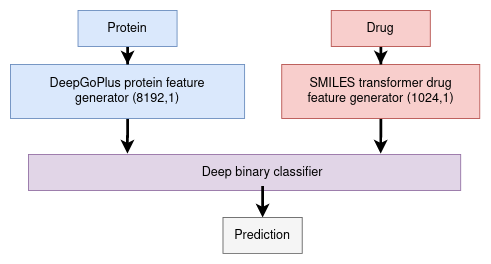
\includegraphics[width=0.4\textwidth]{figures/MolecularPredictor.png}}
% 	\caption{Molecular predictor based on the generated features from DeepGoPlus and SMILES transformer.}\label{fig:MolPred}
% \end{figure}

% \begin{figure}[!tpb]%figure2
% \centerline{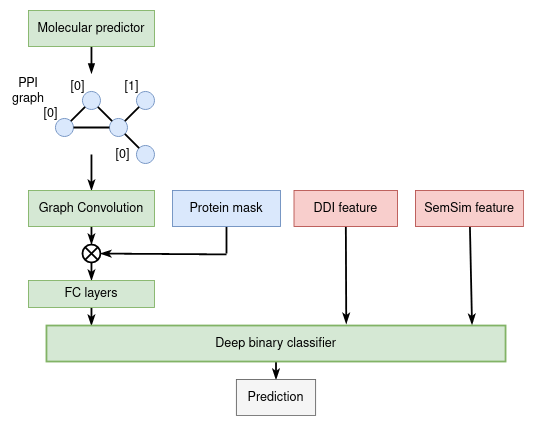
\includegraphics[width=0.4\textwidth]{figures/InteractionNetwork.png}}
% \caption{Deep neural network that predicts based on drug-drug interaction features and semantic similarity features over side effects for drugs, and graph convolution over protein-protein interaction networks for proteins. Protein and drug features are represented by blue and red, respectively.}\label{fig:02}
% \end{figure}

%\section{Discussion}







%%%%%%%%%%%%%%%%%%%%%%%%%%%%%%%%%%%%%%%%%%%%%%%%%%%%%%%%%%%%%%%%%%%%%%%%%%%%%%%%%%%%%
%
%     please remove the " % " symbol from \centerline{\includegraphics{fig01.eps}}
%     as it may ignore the figures.
%
%%%%%%%%%%%%%%%%%%%%%%%%%%%%%%%%%%%%%%%%%%%%%%%%%%%%%%%%%%%%%%%%%%%%%%%%%%%%%%%%%%%%%%






\section{Conclusion}

\vspace*{-10pt}


\section*{Acknowledgements}

\vspace*{-12pt}

\section*{Funding}

This work has been supported by the... Text Text  Text Text.\vspace*{-12pt}

%\bibliographystyle{natbib}
%\bibliographystyle{achemnat}
%\bibliographystyle{plainnat}
%\bibliographystyle{abbrv}
%\bibliographystyle{bioinformatics}
%
%\bibliographystyle{plain}
%
\bibliography{citations}


\end{document}

%%% Local Variables:
%%% mode: latex
%%% TeX-master: t
%%% End:
